%%%%%%%%%%%%%%%%%%%%%%%%%%%%%%%%%%%%%%%%%%%%%%%%%%%%%%%%%%%%%%%%%%%%%%%%%%%%%%%%
%Tutorial slides on Python.
%
% Author: FOSSEE
% Copyright (c) 2009-2016, FOSSEE, IIT Bombay
%%%%%%%%%%%%%%%%%%%%%%%%%%%%%%%%%%%%%%%%%%%%%%%%%%%%%%%%%%%%%%%%%%%%%%%%%%%%%%%%

\documentclass[14pt,compress]{beamer}

% Modified from: generic-ornate-15min-45min.de.tex
\mode<presentation>
{
  \usetheme{Warsaw}
  \useoutertheme{infolines}
  \setbeamercovered{transparent}
}

\usepackage[english]{babel}
\usepackage[latin1]{inputenc}
%\usepackage{times}
\usepackage[T1]{fontenc}

% Taken from Fernando's slides.
\usepackage{ae,aecompl}
\usepackage{mathpazo,courier,euler}
\usepackage[scaled=.95]{helvet}

\definecolor{darkgreen}{rgb}{0,0.5,0}

\usepackage{listings}
\lstset{language=Python,
    basicstyle=\ttfamily\bfseries,
    commentstyle=\color{red}\itshape,
  stringstyle=\color{darkgreen},
  showstringspaces=false,
  keywordstyle=\color{blue}\bfseries}

%%%%%%%%%%%%%%%%%%%%%%%%%%%%%%%%%%%%%%%%%%%%%%%%%%%%%%%%%%%%%%%%%%%%%%
% Macros
\setbeamercolor{emphbar}{bg=blue!20, fg=black}
\newcommand{\emphbar}[1]
{\begin{beamercolorbox}[rounded=true]{emphbar}
      {#1}
 \end{beamercolorbox}
}
\newcounter{time}
\setcounter{time}{0}
\newcommand{\inctime}[1]{\addtocounter{time}{#1}{\tiny \thetime\ m}}

\newcommand{\typ}[1]{\lstinline{#1}}

\newcommand{\kwrd}[1]{ \texttt{\textbf{\color{blue}{#1}}}  }

%%% This is from Fernando's setup.
% \usepackage{color}
% \definecolor{orange}{cmyk}{0,0.4,0.8,0.2}
% % Use and configure listings package for nicely formatted code
% \usepackage{listings}
% \lstset{
%    language=Python,
%    basicstyle=\small\ttfamily,
%    commentstyle=\ttfamily\color{blue},
%    stringstyle=\ttfamily\color{orange},
%    showstringspaces=false,
%    breaklines=true,
%    postbreak = \space\dots
% }

%%%%%%%%%%%%%%%%%%%%%%%%%%%%%%%%%%%%%%%%%%%%%%%%%%%%%%%%%%%%%%%%%%%%%%
% Title page
\title[Interactive Plotting]{Introductory Scientific Computing with
Python}
\subtitle{Introduction, IPython and Plotting}

\author[FOSSEE] {FOSSEE}

\institute[IIT Bombay] {Department of Aerospace Engineering\\IIT Bombay}
\date[] {Mumbai, India
}
%%%%%%%%%%%%%%%%%%%%%%%%%%%%%%%%%%%%%%%%%%%%%%%%%%%%%%%%%%%%%%%%%%%%%%

%\pgfdeclareimage[height=0.75cm]{iitmlogo}{iitmlogo}
%\logo{\pgfuseimage{iitmlogo}}


%% Delete this, if you do not want the table of contents to pop up at
%% the beginning of each subsection:
\AtBeginSubsection[]
{
  \begin{frame}<beamer>
    \frametitle{Outline}
    \tableofcontents[currentsection,currentsubsection]
  \end{frame}
}

\AtBeginSection[]
{
  \begin{frame}<beamer>
    \frametitle{Outline}
    \tableofcontents[currentsection,currentsubsection]
  \end{frame}
}

% If you wish to uncover everything in a step-wise fashion, uncomment
% the following command:
%\beamerdefaultoverlayspecification{<+->}

%%\includeonlyframes{current,current1,current2,current3,current4,current5,current6}

%%%%%%%%%%%%%%%%%%%%%%%%%%%%%%%%%%%%%%%%%%%%%%%%%%%%%%%%%%%%%%%%%%%%%%
% DOCUMENT STARTS
\begin{document}

\begin{frame}
  \maketitle
\end{frame}

%% \begin{frame}
%%   \frametitle{Outline}
%%   \tableofcontents
%%   % You might wish to add the option [pausesections]
%% \end{frame}

\begin{frame}
    \frametitle{Acknowledgement}
    \Large
    \begin{center}
        \alert{FOSSEE group (\url{fossee.in})} \\
        based at\\
        \alert{IIT Bombay}\\
        and funded by\\
        The National Mission on Education through ICT, \\
        \alert{Ministry of HRD, India}
    \end{center}
\end{frame}

\section{Checklist}
\begin{frame}
\frametitle{Checklist}
  \begin{enumerate}
    \item Editor - we recommend \alert{VSCode}
    \item IPython
    \item Data files:
      \begin{itemize}
      \item \typ{pendulum.txt}
      \item \typ{data.csv}
      \end{itemize}
    \item Images
      \begin{itemize}
      \item \typ{penguins.png}
      \end{itemize}
  \end{enumerate}
\end{frame}

\begin{frame}
  \frametitle{About the Tutorial}
  \begin{block}{Intended Audience}
  \begin{itemize}
       \item Engg., Mathematics and Science researchers with a
           reasonable programming background.
  \end{itemize}
  \end{block}

  \begin{block}{Goal: Successful participants will be able to}
    \begin{itemize}
      \item Start using Python as plotting, computational tool.
      \item Use the basic libraries and tools for scientific computing
          with Python.
    \end{itemize}
  \end{block}
\end{frame}

%% \begin{frame}[fragile]
%% \frametitle{The Python interpreter \ldots}
%% \begin{block}{}
%% \begin{lstlisting}
%%   $ python
%% \end{lstlisting} %$
%% \end{block}
%% \begin{lstlisting}
%%   >>> print "Hello, World!"
%%   Hello, World!
%% \end{lstlisting}
%% Exiting
%% \begin{lstlisting}
%%   >>> ^D(Ctrl-D)
%%   $
%% \end{lstlisting} %$
%% \end{frame}

\section{Starting up IPython}
\begin{frame}[fragile]
\frametitle{Starting up \ldots}
\begin{block}{Start a terminal}
  \begin{itemize}
    \item Open Terminal using Anaconda Navigator
\end{itemize}
\end{block}

\begin{block}{On Terminal}
\begin{lstlisting}
  $ ipython --pylab
\end{lstlisting} %$
\end{block}
\end{frame}

% \section{Starting up IPython}
% \begin{frame}[fragile]
% \frametitle{Starting up \ldots}
% \begin{block}{Terminal Jupyter}
% \begin{lstlisting}
%   $ jupyter console

%   In [1]: %pylab
% \end{lstlisting} %$
% \end{block}
% \end{frame}


\begin{frame}[fragile]
\frametitle{Running IPython}
\begin{lstlisting}
  In []: print("Hello, World!")
  Hello, World!
\end{lstlisting}

Exiting on the \textbf{terminal}
\begin{lstlisting}
  In []: ^D(Ctrl-D)
  Do you really want to exit([y]/n)? y
\end{lstlisting}
\end{frame}

\begin{frame}[fragile]
  \frametitle{IPython? }
  \begin{itemize}
  \item An enhanced Python interpreter
  \end{itemize}
\end{frame}

% \begin{frame}[fragile]
%   \frametitle{Pressed Ctrl-D on Canopy? }
%   \begin{itemize}
%   \item Pressed \verb+Ctrl-D+ inside Canopy?
%   \item You suddenly lost the Python prompt?
%   \item Go to \verb+View->Python+
%   \end{itemize}
% \end{frame}


\section{Breaking out of loops}
\begin{frame}[fragile]
\frametitle{Breaking out of Loops}
Breaking out of loops
\begin{lstlisting}
  In []: while True:
    ...:     print("Hello, World!")
    ...:
  Hello, World!
  Hello, World!^C(Ctrl-C)
  ------------------------------------
  KeyboardInterrupt
\end{lstlisting}
\end{frame}

\begin{frame}[fragile]
  \frametitle{Exercise}

  \begin{itemize}
  \item Exit the IPython interpreter
  \item Close the terminal
  \item Restart the terminal
  \item Restart IPython using:
  \end{itemize}
\begin{lstlisting}
  $ ipython --pylab
\end{lstlisting} %$
  \inctime{10}
\end{frame}

\section{Plotting}

\begin{frame}
  \frametitle{Important instructions}
  \begin{itemize}
  \item For the first session, please do not experiment
  \item Follow along and type everything!
  \item Case matters
  \item Every character you type matters!
  \end{itemize}
\end{frame}

\subsection{Drawing plots}
\begin{frame}[fragile]
\frametitle{First Plot}
\begin{columns}
    \column{0.25\textwidth}
    \hspace*{-0.25in}
  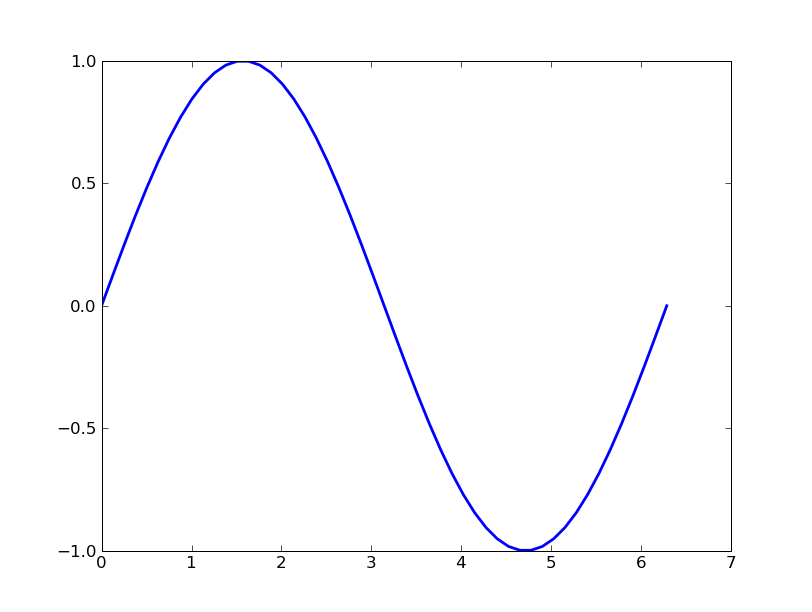
\includegraphics[height=2in, interpolate=true]{data/firstplot}
    \column{0.8\textwidth}
    \begin{block}{}
    \begin{small}
\begin{lstlisting}
In []: x = linspace(0, 2*pi, 50)
In []: plot(x, sin(x))
\end{lstlisting}
    \end{small}
    \end{block}
\end{columns}
\end{frame}

\begin{frame}[fragile]
\frametitle{Walkthrough}
\begin{block}{\typ{x = linspace(start, stop, num)} }
returns \typ{num} evenly spaced points, in the interval [\typ{start}, \typ{stop}].
\end{block}
\vspace*{.35in}
\begin{block}{}
  \small
\begin{lstlisting}
In []: x[0]
Out[]: 0.0

In []: x[49]
Out[]: 6.2831853071795862
\end{lstlisting}
\end{block}
\end{frame}

\begin{frame}[fragile]
\frametitle{Walkthrough \ldots}
\begin{block}{\typ{plot(x, y)}}
plots \typ{x} and \typ{y} using default line style and color
\end{block}
\inctime{5}
\end{frame}

\begin{frame}
  \frametitle{Important instructions}
  \begin{itemize}
  \item Please do not close the plot windows or IPython
  \item For the first session, please do not experiment
  \item Follow along and type everything!
  \item Case matters
  \item Every character you type matters!
  \end{itemize}
\end{frame}

\subsection{Decoration}
\begin{frame}[fragile]
\frametitle{Adding Labels}
\begin{columns}
  \column{0.25\textwidth}
  \hspace*{-0.45in}
  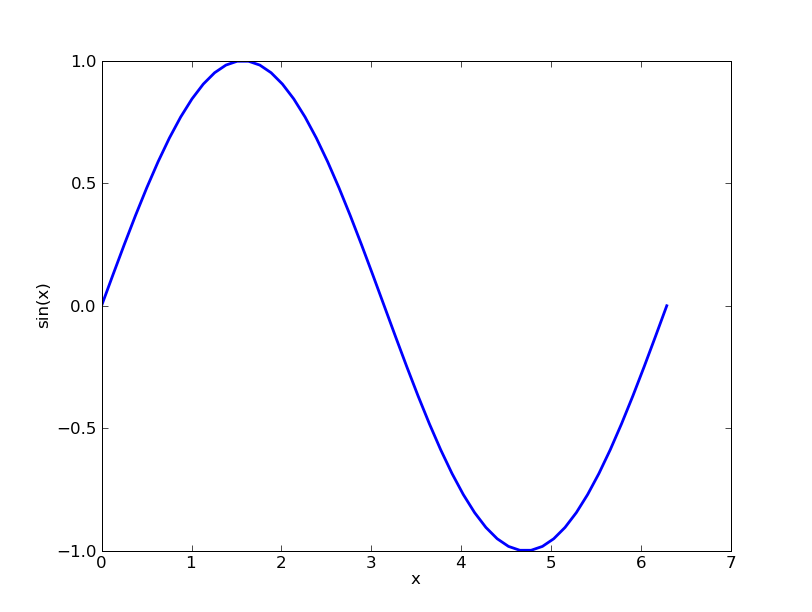
\includegraphics[height=2in, interpolate=true]{data/label}
  \hspace*{0.5in}
  \column{0.55\textwidth}
  \begin{block}{}
  \small
  \begin{lstlisting}
In []: xlabel('x')

In []: ylabel('sin(x)')
  \end{lstlisting}
  \small
%  \end{lstlisting}
%\typ{xlabel(s)} sets the label of the \typ{x}-axis to \typ{s}

%  \begin{lstlisting}
  \end{block}
%\typ{ylabel(s)} sets the label of the \typ{y}-axis to \typ{s}
\end{columns}
\end{frame}

\begin{frame}[fragile]
\frametitle{Another example}
  \begin{lstlisting}
In []: clf()
  \end{lstlisting}
\emphbar{Clears the plot area.}
  \begin{lstlisting}
In []: y = linspace(0, 2*pi, 50)
In []: plot(y, sin(2*y))
In []: xlabel('y')
In []: ylabel('sin(2y)')
  \end{lstlisting}
\end{frame}

\begin{frame}[fragile]
\frametitle{IPython tips}

\begin{itemize}
\item Use \typ{TAB} to complete command
\item Try:
\begin{lstlisting}
In []: pl<TAB>
\end{lstlisting}
\end{itemize}
\vspace*{0.5in}

{\Large \structure{History}}
\begin{itemize}
\item Up arrow and down arrow

\item Left / right to move and edit

\item Type some text and press up arrow:
\begin{lstlisting}
In []: pl<Up Arrow>
\end{lstlisting}

\end{itemize}

\end{frame}

\begin{frame}[fragile]
  \frametitle{Advanced IPython tips \ldots}
  \begin{itemize}
\item Search: \typ{Ctrl-r} and start typing

\item \typ{Ctrl-a}: go to start of line

\item \typ{Ctrl-e}: go to end of line

\item \typ{Ctrl-k}: kill to end of line
  \end{itemize}
\end{frame}


\subsection{More decoration}
\begin{frame}[fragile]
\frametitle{Title and Legends}
\vspace*{-0.15in}
%  \begin{block}{}
%  \small
\begin{lstlisting}
In []: title('Sinusoids')
In []: legend(['sin(2y)'])
\end{lstlisting}
%  \small
%  \end{block}
  \vspace*{-0.1in}
  \begin{center}
  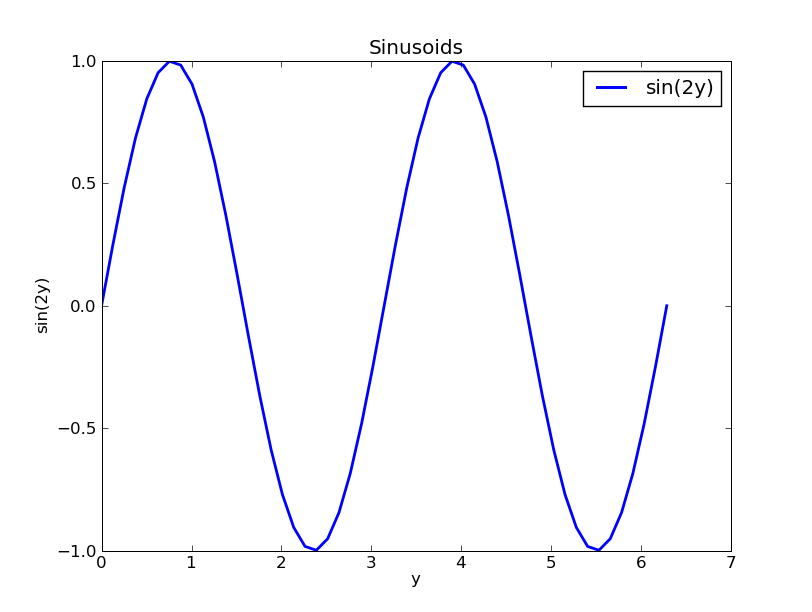
\includegraphics[height=2in, interpolate=true]{data/legend}
  \end{center}
\end{frame}

\begin{frame}[fragile]
\frametitle{Legend Placement}
\begin{block}{}
    \small
\begin{lstlisting}
In []: legend(['sin(2y)'], loc='center')
\end{lstlisting}
\end{block}

\begin{columns}
    \column{0.6\textwidth}
 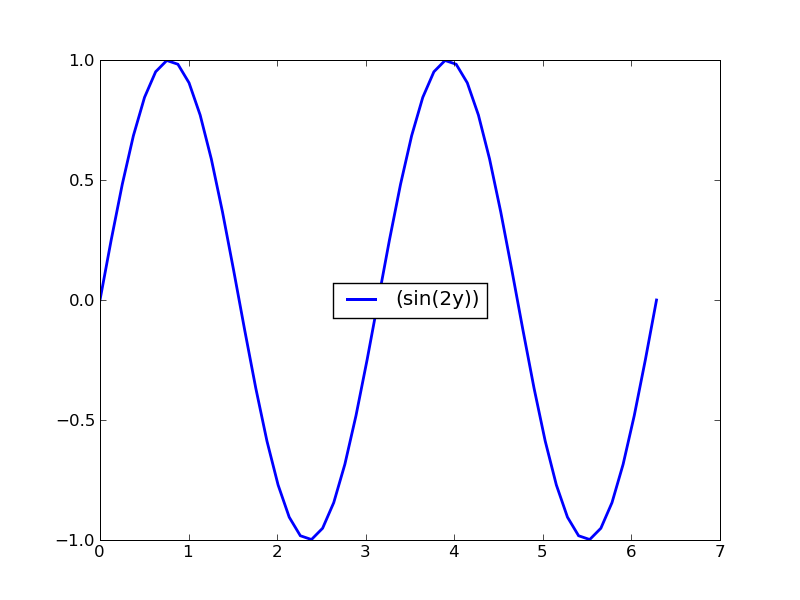
\includegraphics[height=2in, interpolate=true]{data/position}
\column{0.45\textwidth}
\vspace{-0.2in}
\begin{lstlisting}
'best'
'right'
'left'
'center'
\end{lstlisting}
\end{columns}
\inctime{15}
\end{frame}

\begin{frame}
  \frametitle{Important instructions}
  \begin{itemize}
  \item Please do not close the plot windows or IPython
  \item For the first session, please do not experiment
  \item Follow along and type everything!
  \item Case matters
  \item Every character you type matters!
  \end{itemize}
\end{frame}

%% \begin{frame}[fragile]
%%   \frametitle{For arbitrary location}
%% \vspace*{-0.1in}
%% \begin{lstlisting}
%% In []: legend(['sin(2y)'], loc=(.8,.1))
%% \end{lstlisting}
%% \emphbar{Specify south-east corner position}
%% %\vspace*{-0.2in}
%% \begin{center}
%%   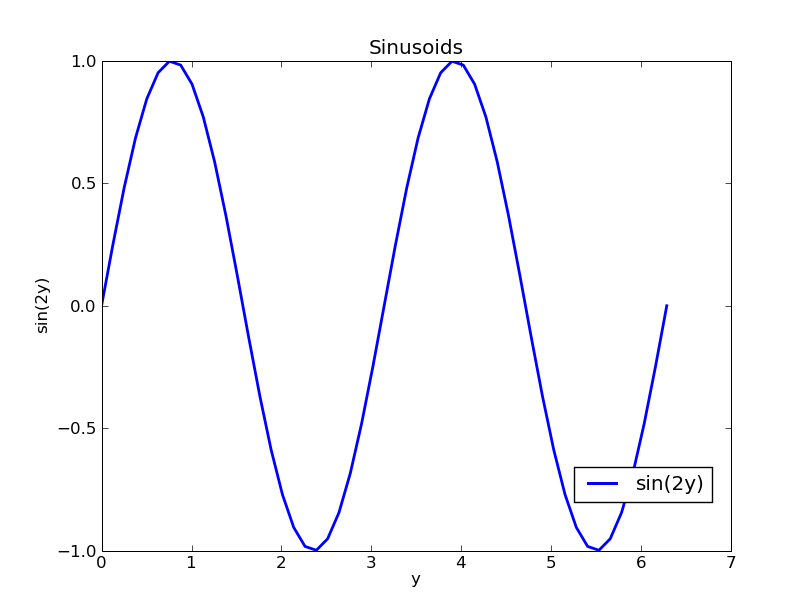
\includegraphics[height=2in, interpolate=true]{data/loc}
%% \end{center}
%% %\inctime{10}
%% \end{frame}

\begin{frame}[fragile]
\frametitle{Showing it better}
\vspace{-0.15in}
\begin{lstlisting}
In []: plot(y, cos(y), 'r')
# See a red plot!

In []: clf()
In []: plot(y, sin(y), 'g', linewidth=2)
\end{lstlisting}
\vspace*{-0.2in}
\begin{center}
  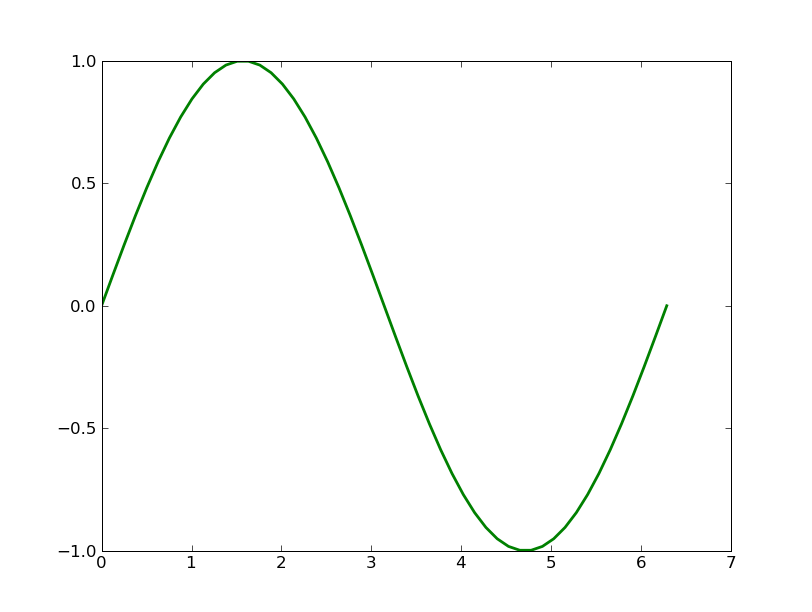
\includegraphics[height=2.2in, interpolate=true]{data/green}
\end{center}
%\inctime{10}
\end{frame}

\begin{frame}[fragile]
\frametitle{Annotating}
\vspace*{-0.1in}
\begin{lstlisting}
In[]: annotate('local max', xy=(1.5, 1))
\end{lstlisting}
\vspace*{-0.2in}
\begin{center}
  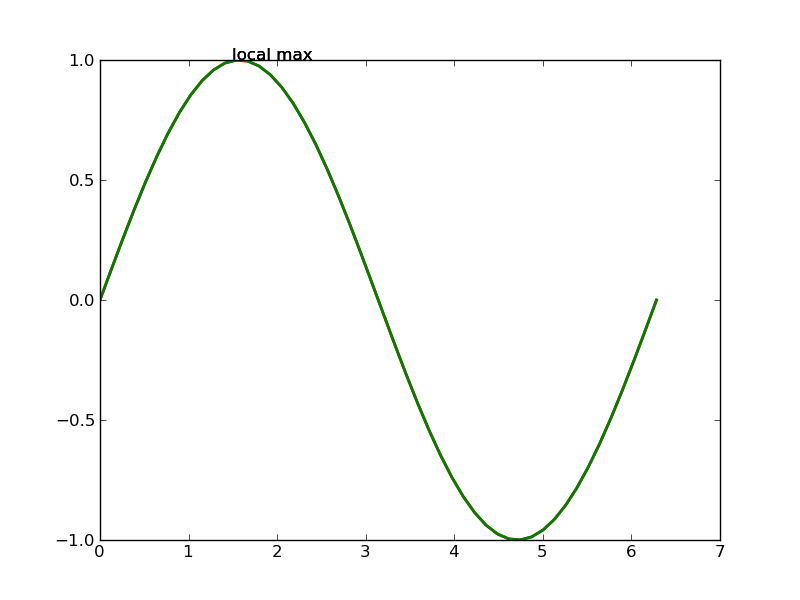
\includegraphics[height=3in, interpolate=true]{data/annotate}
\end{center}
\end{frame}

\begin{frame}[fragile]
\frametitle{Saving \& Closing}
\begin{lstlisting}
In []: savefig('sin.png')

In []: close()
\end{lstlisting}
Some supported formats:
\begin{itemize}
\item png
\item pdf
\item svg
\end{itemize}
\end{frame}

\begin{frame}[fragile]
  \frametitle{Recap}
  \begin{itemize}
  \item \typ{linspace(start, end, num)}
  \item \typ{plot(x, y)}
  \item \typ{clf()}
  \item \typ{xlabel, ylabel}
  \item \typ{title, legend, annotate}
  \item \typ{savefig}
  \item \typ{close}
  \end{itemize}
  \inctime{10}
\end{frame}

\section{Multiple plots}
\begin{frame}[fragile]
  \frametitle{Overlaid Plots}
\begin{lstlisting}
In []: y = linspace(0, 2*pi, 50)
\end{lstlisting}

\begin{lstlisting}
In []: clf()
In []: plot(y, sin(y))
In []: plot(y, cos(y))
In []: xlabel('y')
In []: ylabel('f(y)')
In []: legend(['sin(y)', 'cos(y)'])
# Note how we made two legends
\end{lstlisting}


\emphbar{By default plots would be overlaid!}
\end{frame}

\begin{frame}[fragile]
\frametitle{Plotting separate figures}
\begin{lstlisting}
In []: clf()
In []: figure(1)
In []: plot(y, sin(y))
In []: figure(2)
In []: plot(y, cos(y))
In []: savefig('cosine.png')
In []: figure(1)
In []: title('sin(y)')
In []: savefig('sine.png')
In []: close()
In []: close()
\end{lstlisting}
\end{frame}

\begin{frame}[fragile]
\frametitle{Get Axes lengths}
\emphbar{Getting axes lengths}
  \begin{lstlisting}
In []: xmin, xmax = xlim()
In []: ymin, ymax = ylim()
In []: print(xmin, xmax)
\end{lstlisting}
\pause
\emphbar{Set the axes limits}
  \begin{lstlisting}
In []: xlim(xmin, 2*pi )
In []: ylim(ymin-0.2, ymax+0.2)
  \end{lstlisting}
\end{frame}

\begin{frame}[plain,fragile]
  \frametitle{Axes lengths}
  \vspace*{-0.2in}
  \begin{center}
    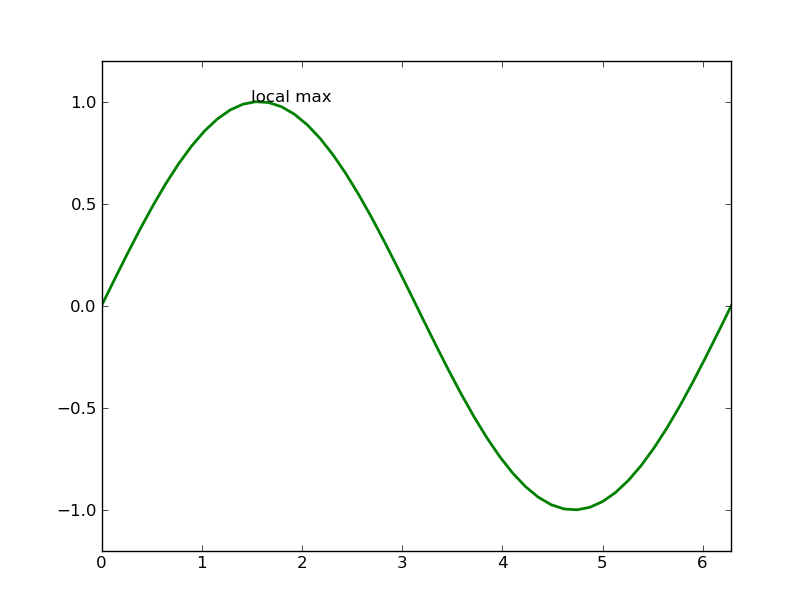
\includegraphics[height=3.25in, interpolate=true]{data/limits}
  \end{center}
\end{frame}

\begin{frame}[fragile]
\frametitle{IPython tip: documentation}

\begin{itemize}

    \item Try:
\begin{lstlisting}
In []: plot?
\end{lstlisting}
      \vspace*{0.2in}
        to get more information on \typ{plot}

      \item Use arrow keys to scroll docs
      \item Note: exit help pager with ``q''
\end{itemize}
\end{frame}

\begin{frame}[fragile]
\frametitle{IPython tip: source}
\begin{itemize}
    \item Try:
\begin{lstlisting}
In []: plot??
\end{lstlisting}
    to see the source code for \typ{plot}

\end{itemize}
\inctime{10}
\end{frame}


\begin{frame}[plain,fragile]
\frametitle{Review Problem}
\begin{enumerate}
\item Plot $x, -x, \sin(x), x \sin(x)$ in range $-5\pi$ to $5\pi$
\item Add a legend
\item Annotate the origin
\item Set axes limits to the range of x
\end{enumerate}
\vspace*{-0.15in}
\begin{center}
  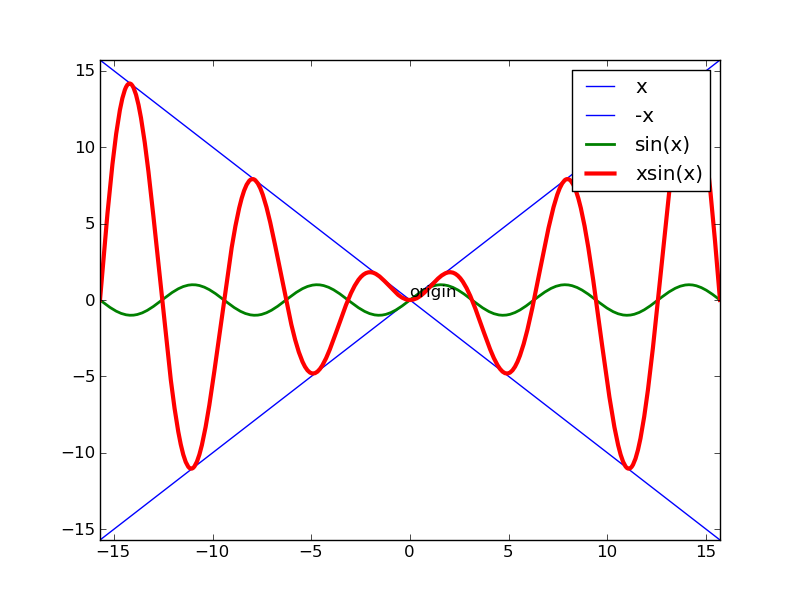
\includegraphics[height=2.6in, interpolate=true]{data/four_plot}
\end{center}
\end{frame}

\end{document}
